\SourcePage{639}{642}
\section{The dispersion relation}

In the preceding section we studied the analytic properties of partial
scattering amplitudes for specified values of $l$. We saw that these
properties are complicated by the possible appearance of ``extraneous''
singularities and by irregularity at infinity. Evidently the total amplitude,
regarded as a function of energy at a specified scattering angle, has the same
properties. The amplitude for scattering through zero angle is an exception,
however. As we shall now show, its analytic properties are considerably
simpler.

Write the Schrödinger equation for the wave function of the scattered particle
as
\begin{equation}
 \Delta\psi+k^2\psi=\frac{2mU}{\hbar^2}\psi,
 \tag{129.1}
\end{equation}
and regard it formally as a wave equation with a right-hand side, that is, as
the retarded-potential equation familiar from electrodynamics.

The solution of this equation describing ``radiation'' in a direction
$\mathbf k'$ at large distances $R_0$ from the center has, as is known, the
following form (see II, \S~66):
\begin{equation}
 \psi_{\mathrm{sc}}=-\frac1{4\pi}\frac{e^{ikR_0}}{R_0}
 \int\frac{2mU}{\hbar^2}\psi e^{-i\mathbf k'\mathbf r}dV.
 \tag{129.2}
\end{equation}

\SourcePage{640}{643}
Here this expression is the wave function of the scattered particle, and the
coefficient of $e^{ikR_0}/R_0$ is the scattering amplitude $f(\theta,E)$. In
particular, putting $\mathbf k'=\mathbf k$, where $\mathbf k$ is the wave
vector of the incident particle, gives the amplitude for scattering through
angle zero:
\begin{equation}
 f(0,E)=-\frac{m}{2\pi\hbar^2}\int U\psi e^{-ikz}dV
 \tag{129.3}
\end{equation}
(the $z$ axis is directed along $\mathbf k$). This expression has, of course,
only a formal meaning, since the unknown wave function again occurs in the
integrand. It nevertheless permits definite conclusions concerning the
analytic properties of $f(0,E)$ as a function of the energy
$E$\footnote{It is understood, of course, that the field $U(r)$ decreases
sufficiently rapidly as $r\to\infty$ for $f(0,E)$ to exist at all when $E>0$
(see \S~124).}.

At large $r$, the function $\psi$ under the integral sign consists of two
parts, an incident wave and an outgoing wave. The latter is proportional to
$e^{ikr}$, so that the corresponding part of the integrand contains
$e^{ik(r-z)}$. On continuation into the complex plane from the upper edge of
the cut along the positive real semiaxis, $ik$ is replaced by
$-\sqrt{-2mE}/\hbar$, and throughout the physical sheet
$\operatorname{Re}\sqrt{-E}>0$. Since $r\geqslant z$, it follows that
$\operatorname{Re}[ik(r-z)]<0$, and the integral converges for every complex
$E$. As for the incident wave in $\psi$, which is proportional to $e^{ikz}$,
the exponential factors in the corresponding part of the integral cancel
altogether, and this part also converges.

For every complex $E$, the function $\psi$ in (129.3) is uniquely determined
as the solution of the Schrödinger equation which, besides the plane wave,
contains only a part that decays as $r\to\infty$. The entire convergent
integral (129.2) is therefore uniquely determined, and its singularities can
arise only when $\psi$ becomes infinite. This occurs at the discrete energy
levels\footnote{To avoid misunderstanding, we emphasize that the function in
question here is the total wave function $\psi$ of the system, normalized by
requiring the coefficient of the plane wave in its asymptotic expression to
be unity (compare (123.3)). In the preceding section, however, the parts
$\psi_l$ of the wave function corresponding to specified values of $l$ were
considered, and each $\psi_l$ was assumed to be normalized by an arbitrary
condition. If the total function $\psi$ is expanded in the functions
$\psi_l$, the latter enter $\psi$ with coefficients proportional to $1/B_l$;
thus the function (128.3) with $l=0$
\[
 \text{must enter }\psi\text{ in the form}\qquad
 \frac{\mathrm{const}}r\frac1B[(A+B)e^{ikr}-2iB\sin kr].
\]
Hence $\psi$ becomes infinite at the zeros of $B_l(E)$, that is, at the
discrete energy levels.}.

\SourcePage{641}{644}
It is also readily seen that $f(0,E)$ remains finite as $|E|\to\infty$. At
large $|E|$, the term containing $U$ may be neglected in the Schrödinger
equation (129.1), leaving only the plane wave in $\psi$:
$\psi\sim e^{ikz}$. The integral (129.2) then becomes
\[
 f(0,\infty)=-\frac{m}{2\pi\hbar^2}\int U\,dV,
\]
which, as it should, agrees with the Born amplitude (126.4) for scattering
through zero angle ($q=0$); denote it by $f_B(0)$.

We thus conclude that the amplitude for scattering through zero angle is
regular throughout the physical sheet, including infinity, except only for
the necessary poles on the negative real semiaxis at the discrete energy
levels\footnote{The idea of this proof is due to L.~D.~Faddeev (1958).}.

Consider the integral
\begin{equation}
 \frac1{2\pi i}\int_C\frac{f(0,E')-f_B}{E'-E}\,dE',
 \tag{129.4}
\end{equation}
taken over the contour shown in Fig.~46, which consists of a circle at
infinity and a circuit around the cut along the positive semiaxis. The
integral over the circle vanishes, since $f(0,\infty)-f_B=0$. Integration
along the two sides of the cut gives
\[
 \frac1\pi\int_0^\infty\frac{\operatorname{Im}f(0,E')}{E'-E}\,dE';
\]
here we have used the fact that, according to the definition adopted in
\S~128, the physical scattering amplitude for real positive $E$ is specified
on the upper side of the cut, while on the lower side it has the
complex-conjugate value.

\begin{figure}[htbp]
\centering
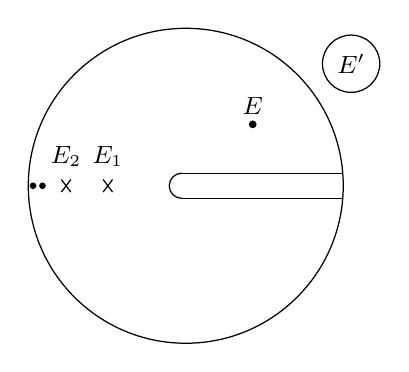
\begin{tikzpicture}[x=1cm,y=1cm,>=stealth,line width=.45pt,font=\small]
 \draw (-2.0,0) arc[start angle=180,end angle=-180,radius=2.0];
 \draw (-.05,.16)--(2.0,.16); \draw (2.0,-.16)--(-.05,-.16);
 \draw (-.05,.16) arc[start angle=90,end angle=270,radius=.16];
 \fill (0.85,.78) circle (1.4pt) node[above] {$E$};
 \draw (-1.05,0.08)--(-.93,-.08); \draw (-1.05,-.08)--(-.93,.08);
 \node[above] at (-.99,.12) {$E_1$};
 \draw (-1.58,0.08)--(-1.46,-.08); \draw (-1.58,-.08)--(-1.46,.08);
 \node[above] at (-1.52,.12) {$E_2$};
 \fill (-1.82,0) circle (1.2pt); \fill (-1.94,0) circle (1.2pt);
 \node[circle,draw,inner sep=3pt] at (2.1,1.55) {$E'$};
\end{tikzpicture}
\caption{}
\label{fig:46}
\end{figure}

On the other hand, Cauchy's theorem says that the integral (129.4) is equal
to the sum of $f(0,E)-f_B$ and the residues $R_n$ of the integrand at all the
poles $E'=E_n$ of $f(0,E')/(E'-E)$,

\SourcePage{642}{645}
where $E_n$ are the discrete energy levels. These residues are determined by
(128.17) and are
\begin{equation}
 R_n=\frac{d_n}{E_n-E},\qquad
 d_n=-(-1)^{l_n}(2l_n+1)\frac{\hbar^2A_{0n}^2}{2m}
 \tag{129.5}
\end{equation}
($l_n$ is the angular momentum of the state of energy $E_n$).

Thus we obtain
\begin{equation}
 f(0,E)=f_B+\frac1\pi\int_0^\infty\frac{\operatorname{Im}f(0,E')}{E'-E}\,dE'
 +\sum_n\frac{d_n}{E-E_n}.
 \tag{129.6}
\end{equation}
This is the so-called \emph{dispersion relation}. It determines $f(0,E)$ at
any point of the physical sheet from the values of its imaginary part for
$E>0$ (D.~Wong, 1957; N.~N.~Khuri, 1957).

As the point $E$ approaches the upper side of the cut, the integral along the
real axis in (129.6) must be taken with the pole $E'=E$ bypassed from below.
If this bypass is made along an infinitesimal semicircle (Fig.~47), the
corresponding part of the integral contributes
$i\operatorname{Im}f(0,E)$ to the right-hand side of (129.6), while the
remaining integral from zero to infinity must be understood as a principal
value. We thereby obtain

\begin{figure}[htbp]
\centering
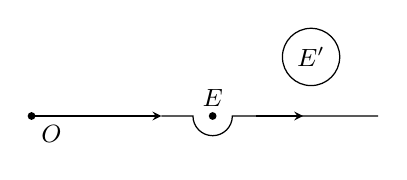
\begin{tikzpicture}[x=1cm,y=1cm,>=stealth,line width=.45pt,font=\small]
 \draw[->] (-2.3,0)--(-.65,0);
 \draw (-.65,0)--(-.25,0) arc[start angle=180,end angle=360,radius=.25]--(2.1,0);
 \draw[->] (.55,0)--(1.15,0);
 \fill (-2.3,0) circle (1.4pt) node[below right] {$O$};
 \fill (0,0) circle (1.4pt) node[above] {$E$};
 \node[circle,draw,inner sep=3pt] at (1.25,.75) {$E'$};
\end{tikzpicture}
\caption{}
\label{fig:47}
\end{figure}

\begin{equation}
 \operatorname{Re}f(0,E)=f_B+\frac1\pi\,\mathrm{P}\!\int_0^\infty
 \frac{\operatorname{Im}f(0,E')}{E'-E}\,dE'+\sum_n\frac{d_n}{E-E_n},
 \tag{129.7}
\end{equation}
which, for $E>0$, determines the real part of the zero-angle scattering
amplitude from its imaginary part. Recall that the latter is directly related
to the total scattering cross-section by (125.9).
